\documentclass[11pt,a4paper]{article}
\usepackage[utf8]{inputenc}\usepackage[T1]{fontenc}
\usepackage[margin=1in]{geometry}
\usepackage{amsmath,amssymb,booktabs,array,graphicx,enumitem,xcolor,parskip,titlesec}
\usepackage[hidelinks]{hyperref}
\graphicspath{{figures/}}
\definecolor{qnavy}{RGB}{20,40,75}\definecolor{qgrey}{RGB}{90,90,90}\definecolor{qred}{RGB}{150,30,30}
\titleformat{\section}{\large\bfseries\color{qnavy}}{\thesection}{0.6em}{}
\input{MACROS.tex}
\emergencystretch=2em
\begin{document}\thispagestyle{empty}
\noindent
{\large\bfseries\color{qnavy} Report R12 --- Federated Learning Across Simulated Hospital Silos}\\[2pt]
{\color{qgrey}What single-site training misses, what federation recovers, and what it costs to move
--- measured on five TCGA pseudo-hospitals with CPTAC-independent machinery.}\\[6pt]
{\color{qgrey}\rule{\textwidth}{0.4pt}}

\medskip
\noindent 11 August 2026 \quad\textbullet\quad Quantara \quad\textbullet\quad
NSCLC RWPR study, Arm C

\section*{Summary}

We split the TCGA-LUAD/LUSC slide cohort (\RPatientsKept{} patients, \RSlidesKept{} whole-slide
images, Phikon-v2 features) into \RNSilos{} pseudo-hospitals anchored on real tissue-source
sites, then trained the same attention-MIL model under the regimes a hospital consortium would
actually choose between: each site alone, federated averaging (weights only cross the boundary),
and the centralized pool-everything upper bound. Every number below is extracted mechanically
from the evidence bundle by \texttt{extract\_numbers.py}; the config was SHA-256-hashed before
any label value was read (\texttt{\RConfigShaShort}\ldots).

\textbf{Single-site models look perfect at home and are not.} On its own site's validation
patients, every local subtype model scores AUROC \RSubtypeDiagMean. Carried to the other four
sites, the same models average \textbf{\RSubtypeOffdiagMean} with a worst case of
\textbf{\RSubtypeOffdiagWorst} --- below chance. The features carry a strong site signature (a
linear probe identifies the silo of a slide at balanced accuracy \RProbeBalAcc{} against a
\RProbeChance{} chance rate, permutation $p=\RProbeP$), and a single-site model happily uses it.

\textbf{Federation recovers the pooled-data result without pooling the data.} FedAvg reaches
subtype AUROC \textbf{\RSubtypeFedavgMean} (\RSubtypeFedavgLo--\RSubtypeFedavgHi) against the
centralized upper bound of \RSubtypeCentralMean{} (\RSubtypeCentralLo--\RSubtypeCentralHi), and
is likewise within the centralized confidence interval on EGFR and OS. The pre-registered
FedProx fallback was never triggered.

\textbf{The cost of that is \RRunTotalMiB{} MiB of model weights} per full federated run
(\RRounds{} rounds $\times$ \RNSilos{} silos $\times$ both directions, \RRoundMiB{} MiB per
round, logged per silo per round in \texttt{evidence/transfer\_log.json}) --- versus
\RRawGiB{} GiB if the training \emph{feature tensors} were centralized instead:
\textbf{\RRawOverFed$\times$ less transfer}, before even counting the raw pixels those features
came from. No image, feature, or label ever crossed a silo boundary.

All \RNGates{} pre-declared gates pass. This is a simulation with one honest limitation, stated
in \S6: TCGA site groups are cohort-disjoint, which makes the site shortcut here as extreme as
it can be.

\section{Design}

\begin{itemize}[leftmargin=1.2em,itemsep=2pt]
\item \textbf{Silos.} TCGA tissue-source-site (TSS) codes are cohort-disjoint (no TSS contributed
both LUAD and LUSC), so each pseudo-hospital pairs one LUAD site-group with one LUSC site-group,
greedily balanced by patient count. All slides of a patient live in exactly one silo.
\item \textbf{Regimes on identical splits} (per seed, 80/20 within each silo; the union of silo
validation sets is \emph{the} pooled validation set for every regime): (1) local single-silo
models, (2) FedAvg (\RRounds{} rounds, 2 local epochs/round, patient-count-weighted averaging),
(3) FedProx, pre-registered to run only if FedAvg diverged or trailed centralized by
$>$5\,pp subtype AUROC (it did neither --- observed gap $-$0.6\,pp, i.e.\ FedAvg ahead), and
(4) centralized training on the pooled data as the upper bound.
\item \textbf{Endpoints.} LUAD-vs-LUSC subtype ($n=\RNSubtype$), EGFR mutation
($n=\RNEgfr$; \REgfrMutants{} mutants), OS ($n=\RNOs$, \RNOsEvents{} events, Cox
partial-likelihood head, Harrell C).
\item \textbf{Model and execution.} Gated attention-MIL over 1024-d Phikon-v2 tile features;
each silo's local step ran in its own Modal container; only serialized \texttt{state\_dict}s
crossed containers, logged byte-for-byte both directions. \RNSeeds{} seeds throughout; CIs are
mean $\pm$ 1.96\,SD$/\sqrt{n_\text{seeds}}$.
\item \textbf{Pre-registration.} \texttt{evidence/config.yaml}, SHA-256
\texttt{\RConfigShaShort\ldots} (full hash embedded in \texttt{results.json}), written before
any label value was read; the config's declared schema-only reads are itemized in the file.
\end{itemize}

\begin{center}
\input{generated_silo_table}
\end{center}

\noindent{\small One bookkeeping discrepancy, reported rather than hidden: the pre-registered
config's \texttt{patients\_kept} field says \RPatientsKeptConfig, but the four QC-excluded
slides were the only slide of four patients, so \RPatientsKept{} patients actually enter the
silos --- the count carried consistently by \texttt{silos.json} and \texttt{results.json}.}

\section{The site shortcut}

\begin{center}
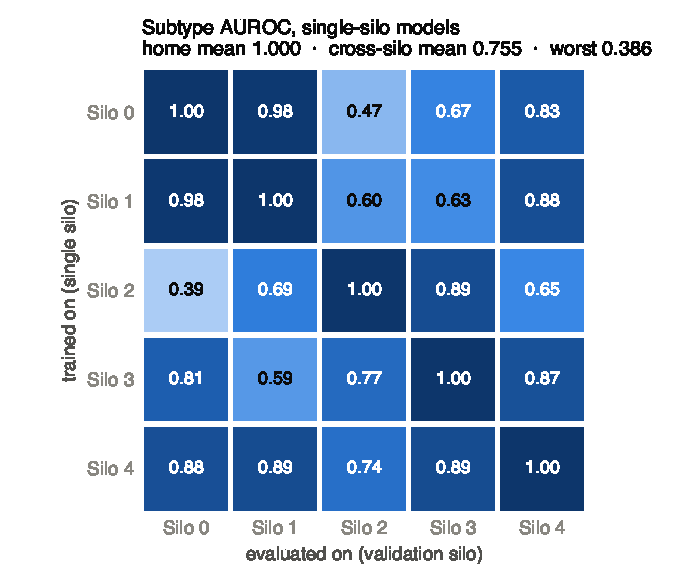
\includegraphics[width=0.62\textwidth]{fig_cross_silo.pdf}
\end{center}
\noindent{\small\color{qgrey}Seed-mean subtype AUROC of each single-silo model (rows) on each
silo's validation patients (columns). Diagonal = home site.}

Every local model is perfect at home (\RSubtypeDiagMean) and averages \RSubtypeOffdiagMean{}
away from home; the worst cell is \RSubtypeOffdiagWorst, \emph{below chance} --- the silo-2
model's site shortcut actively inverts on silo 0. The mechanism is measured, not conjectured:
silo identity is linearly decodable from the mean tile embedding at balanced accuracy
\RProbeBalAcc{} (chance \RProbeChance, permutation $p=\RProbeP$ over \RProbeNPerm{} shuffles).
Because each pseudo-hospital's LUAD and LUSC come from different real sites, scanner and stain
are partially aligned with the label within a silo --- a model can score perfectly at home
while learning the wrong thing. The cross-silo row is what deployment at a new hospital
would see.

\section{What federation buys, in practice}

\begin{center}
\small
\input{generated_practice_table}
\end{center}
\noindent{\small\color{qgrey}Seed-mean over \RNSeeds{} seeds (95\% CI); all regimes scored on
the identical pooled validation set. ``Local, home'' scores each validation patient with their
own site's model; ``Local, other silos'' averages each single-site model over the full pooled
set.}

\begin{center}
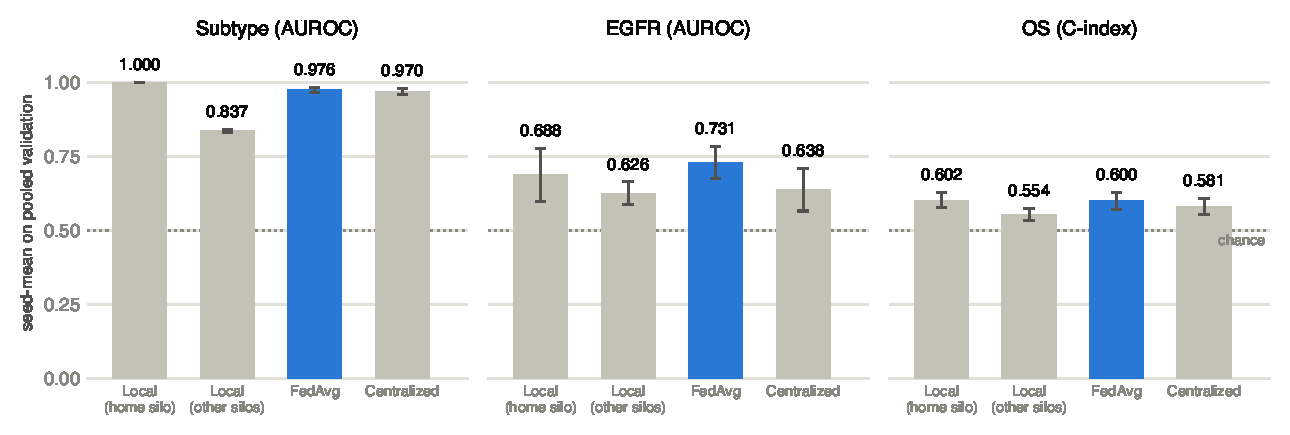
\includegraphics[width=\textwidth]{fig_regimes.pdf}
\end{center}

On subtype, FedAvg closes the entire deployment gap: from \RSubtypeLocalGlobalMean{} (local
models on other sites' patients) to \RSubtypeFedavgMean, statistically indistinguishable from
--- numerically slightly above --- the centralized \RSubtypeCentralMean. On EGFR and OS the
centralized-vs-local gap is itself within seed noise, so no ``fraction of gap recovered'' is
claimed there; the honest statement is that \textbf{FedAvg is never worse than the best
alternative on any endpoint} (EGFR \REgfrFedavgMean{} vs centralized \REgfrCentralMean; OS
C-index \ROsFedavgMean{} vs \ROsCentralMean), while never moving data. EGFR and OS are weak
signals for every regime; see the power statement in \S5.

\section{Communication cost}

\begin{center}
\begin{tabular}{@{}lr@{}}
\toprule
Serialized model per direction (one silo, one round) & \RStateDictBytes{} bytes ($\approx$ \RStateDictMiB{} MiB) \\
One round, all \RNSilos{} silos, both directions & \RRoundMiB{} MiB \\
One complete FedAvg run (\RRounds{} rounds) & \textbf{\RRunTotalMiB{} MiB} \\
Training feature tensors, if centralized instead & \RRawGiB{} GiB \\
\midrule
Ratio & \textbf{\RRawOverFed$\times$} \\
\bottomrule
\end{tabular}
\end{center}

\noindent Every byte is logged per silo per round in \texttt{evidence/transfer\_log.json}
(\RNFedavgRunsLogged{} runs $\times$ \RRounds{} rounds); the totals above are re-summed from
that log by \texttt{extract\_numbers.py}, not copied. The \RRawGiB{} GiB comparator is the
Phikon-v2 \emph{feature} spine --- itself orders of magnitude smaller than the source WSI
pixels --- so \RRawOverFed$\times$ understates the saving against shipping images. Total
simulation cost: $\approx$\,\$\RCostUsd{} of Modal GPU time.

\section{Gates and power}

All \RNGatesPass{} gate-carrying checks pass; the FedProx trigger is recorded as evaluated and
not fired. The EGFR permutation null (\RPermNullN{} label-shuffled centralized runs) is centred
at \RPermNullMean.

\begin{center}
\small
\input{generated_gates_table}
\end{center}

\noindent\textbf{EGFR power, stated in full (gate \texttt{g7}):} \input{generated_power_statement}

\section{Honest caveats}

\begin{itemize}[leftmargin=1.2em,itemsep=2pt]
\item \textbf{The site shortcut is at its most extreme here.} TCGA sites are cohort-disjoint,
so within a pseudo-hospital the site signature is partially aligned with the subtype label by
construction. Real hospitals see both subtypes; their local models would degrade less
dramatically than \RSubtypeOffdiagWorst. The direction of the effect --- local models
overstate themselves at home, federation restores cross-site validity --- is the transferable
finding, not the magnitude.
\item \textbf{EGFR and OS are weak for every regime.} With \REgfrMutants{} mutants the EGFR
endpoint can only resolve AUROC $\geq \REgfrMde$; OS C-indices sit near
\ROsCentralMean{}--\ROsFedavgMean{} for all regimes. Neither endpoint is claimed as a win for
any regime; they are carried to show federation does not \emph{hurt} hard endpoints.
\item \textbf{This is a simulation of the deployment topology, not of hospital IT.} One
container per silo with weights-only exchange reproduces the data-flow constraint; it does not
test a real firewall, scheduler, or governance process.
\end{itemize}

\section{Reproducing this report}

\begin{itemize}[leftmargin=1.2em,itemsep=1pt]
\item Every number: \texttt{python3 extract\_numbers.py} regenerates \texttt{MACROS.tex} and
all table bodies from \texttt{evidence/}; figures: \texttt{python3 make\_figures.py}.
\item Any AUROC can be recomputed from the out-of-fold files, e.g.
\begin{quote}\small\begin{verbatim}
python3 -c "
import numpy as np; from sklearn.metrics import roc_auc_score
d=np.loadtxt('evidence/oof_subtype_fedavg_seed0.csv',
             delimiter=',',skiprows=1,usecols=(2,3))
print(roc_auc_score(d[:,0].astype(int), d[:,1]))"
\end{verbatim}\end{quote}
\item Evidence bundle: verbatim copy of \texttt{nsclc-rwpr-study/armC/evidence/} (run of
2026-08-10), plus \texttt{config.yaml} whose SHA-256 equals the \texttt{config\_sha256} inside
\texttt{results.json}. Original run artifacts:
\texttt{gs://heydonto-quantara-lungcdx/nsclc-rwpr-study/armC/runs/}.
\end{itemize}

\end{document}
